%%%%%%%%%%%%%%%%%%%%%%%%%% author.tex %%%%%%%%%%%%%%%%%%%%%%%%%
%
% sample root file for your contribution to an IFIP volume
% published at Springer
%
% Use this file as a template for your own input.
%
%%%%%%%%%%%%%%%%%%%%%%%% Springer-Verlag %%%%%%%%%%%%%%%%%%%%%%%%%%


% RECOMMENDED %%%%%%%%%%%%%%%%%%%%%%%%%%%%%%%%%%%%%%%%%%%%%%%%%%%
\documentclass[ifip]{svmult}
\usepackage{fancyvrb,xcolor}
\usepackage{alltt}

% choose options for [] as required from the list
% in the Reference Guide, Sect. 2.2
\usepackage{url}
\usepackage{epsfig}
\usepackage{makeidx}         % allows index generation
\usepackage{graphicx}        % standard LaTeX graphics tool
                             % when including figure files
\usepackage{multicol}        % used for the two-column index
\usepackage[bottom]{footmisc}% places footnotes at page bottom
\usepackage{float}           % H para posicionar figuras
\usepackage{booktabs}
\usepackage{color}

% etc.
% see the list of further useful packages
% in the Reference Guide, Sects. 2.3, 3.1-3.3

\makeindex             % used for the subject index
                       % please use the style sprmidx.sty with
                       % your makeindex program


%%%%%%%%%%%%%%%%%%%%%%%%%%%%%%%%%%%%%%%%%%%%%%%%%%%%%%%%%%%%%%%%%%%%%

\begin{document}

\title*{Analyzing how the bugs are injected into the source code.}
% Use \titlerunning{Short Title} for an abbreviated version of
% your contribution title if the original one is too long
\author{Gema Rodr\'iguez-P\'erez\inst{1}}
%\and Name of Author\inst{2}}
% Use \authorrunning{Short Title} for an abbreviated version of
% your contribution title if the original one is too long,
\institute{\texttt{gerope@libresoft.es}, LibreSoft, Universidad Rey Juan Carlos}
%
% Use the package "url.sty" to avoid
% problems with special characters
% used in your e-mail or web address
%
\maketitle

\begin{abstract}
There is an ample research in the software engineering literature on software defects. In the field of mining software repositories, it's very important understand how the bugs are injected into the source code to prevent the system to fail. In the currently literature many studies on bug seeding start with an implicit assumption: the bug fixed had been introduced in the previous modification (i.e., in the previous commit) of those same lines of the source code. However, we have conducted and observational study that proved the assumption that bugs have been introduced in the previous commit and the results, showed this assumption does not hold for a large fraction of the bugs analyzed.

Our objective is shed some light on bug seeding topic by analyzing how the bug are inserted into the source code and understanding why the bug appears in the source whereas the developers are at their disposal code reviews and automatic inspections. We pretend conducted an large observational study that involved bug notifications from a free and open-source cloud computing software platform in order to find some pattern that can help us preventing the bugs. 
\end{abstract}

\keywords{Bug introduction, bug seeding, SZZ algorithm, previous commit}

\section{Introduction}
\label{sec:1}

Many efforts on how and why bugs are introduced in the software source code are underway in the software engineering research community. Software source code is affected by many changes, many of them due to failure of the software because of emergent bugs. Developers try to fix them by locating and modifying the line(s) of source code in which the bug is. Concepts such as \emph{bug seeding} help us to find how and where a bug was inserted in the source code, and should be reasonable to assume that last modification, or \textit{previous commit}, of this line or these lines injected the bug.

In spite of the many studies in the area of mining software repositories that are based on this implicit assumption, it is not a trivial task to find when and where a bug has been introduced in the source code, and thus to identify who introduced the bug. There are some reasons to assume that in some cases the bug may not have been introduced in the previous commit, being other actions such as change in the API that is being called or an older modification the cause for a bug. But in fact, this has been largely ignored in the related work; as anecdotal evidence in papers of different areas of research the following statements can be found: 

\begin{itemize}
  \item in bug seeding studies, e.g., \textit{``This earlier change is the one that caused the later fixed''}~\cite{williams2008szz} or \textit{``The lines affected in the process of fixing a bug are the same one that originated or seeded that bug''}~\cite{izquierdo2011developers},
  \item in bug fix patterns, e.g., \textit{``The version before the bug fix revision is the bug version''}~\cite{pan2009toward},
  \item in tools that prevent future bugs, e.g., \textit{``We assume that a change/commit is buggy if its modifications has been later altered by a bug-fix commit''}~\cite{fejzer2015supporting}. 
\end{itemize}

While performing research on the topic, the unique empirical evidence found in the literature that supports this assumption is based on a manual verification of 25 random bug-fix commits with some improvements in the use of the SZZ algorithm, concluding that the SZZ intuition in which the change previous to a bug fix introduces the bug is fulfilled~\cite{williams2008szz}. But this empirical evidence is not enough, it only takes a small population of bug-fix commits, and we need more empirical evidence because of the assumption can be found frequently in the literature. That is the reason why we decided to investigate its validity in the case of a large project, such as the OpenStack, pinpointing the origin of a bug in the source code and devoting significant effort to understand the causes. 

The many changes to the code in this project enables us to identify bug reports in which the bug had not been introduced in the previous commit. As we have mentioned before, an example of this could be a change in the API that is being called. For instance, the code presented below shows a real code extracted from OpenStack in which a certain volume doesn't work with multiple backend enable, due to in the current design it was not necessary, see red lines in \textit{Bug-Insertion (V2)}, but in a certain moment and for some reasons, the community need it. So, the fixed bug added a new value in API call, see green lines in \textit{Bug-Fix (V5):}. 

The Figure 1 shows an example of the history of commits done in a file, we can see the current version, \textit{V6}, the commit that fix the bug, \textit{V5}, the commit that injected the bug according with SZZ intuition, \textit{V2}. The commit \textit{V1} is the first time that the function involved in the bug fix appear in the file, and the commits \textit{V3,V4} are different states of the file. 

\begin{figure}[ht]
\centering
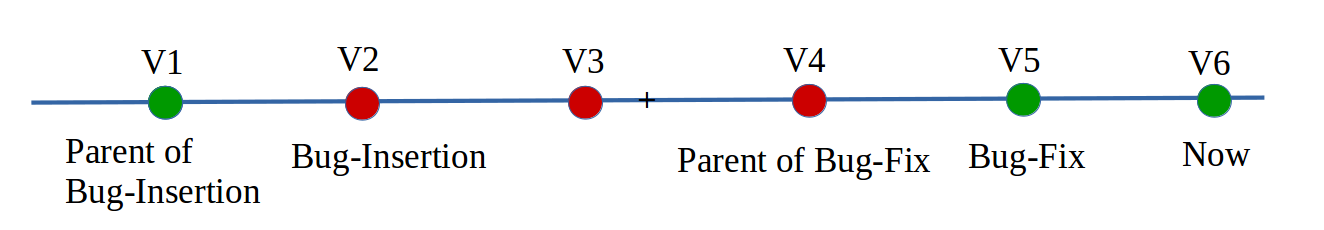
\includegraphics[height=2cm]{History.png}
\caption{Control version history with the bug-insertion commit and the bug-fix commit }
\label{fig:history}       % Give a unique label
\end{figure}

Before Bug-Insertion (V1):
\begin{Verbatim}[fontsize=\small,commandchars=\\\(\)]
	dbb854635 xioaxi 2013-07-11	def _check_backup_service {self,volume}:
	afd69a95b victor 2013-08-28	"""Check if there us an backup service available."""
	dbb854635 xioaxi 2013-07-11	topic = CONF.backup_topic
		...				...
	dbb854635 xioaxi 2013-07-11		srv['host']==volume['host'] and not srv['disable']
 \end{Verbatim}

 Bug-Insertion (V2): 
\begin{Verbatim}[fontsize=\small,commandchars=\\\(\)]
	(\color(red)d6dd5cdfa keniche 2013-09-05	def _is_backup_service_enabled {self,volume}:)
	afd69a95b victor 2013-08-28	"""Check if there us an backup service available."""
	dbb854635 xioaxi 2013-07-11	topic = CONF.backup_topic
		...				...
	(\color(red)dbb854635 xioaxi 2013-07-11		srv['host']==volume['host'] and not srv['disable'])
 \end{Verbatim}

Bug-Fix (V5): 
\begin{Verbatim}[fontsize=\small,commandchars=\\\(\)]
	(\color(green)bd5c3f5a0 Edward 2013-09-26	def _is_backup_service_enabled{self,volume,volume_host}:)
	afd69a95b victor 2013-08-28	"""Check if there us an backup service available."""
	dbb854635 xioaxi 2013-07-11	topic = CONF.backup_topic
		...				...
	(\color(green)bd5c3f5a0 Edward 2013-09-26		srv['host']==volume_host and not srv['disable'])
 \end{Verbatim}

In this example, according to SZZ algorithm the previous commits \textit{d6dd5cdfa and dbb854635} inserted the bug; due to some drawbacks in this algorithm, the approach carried on~\cite{kim2006automatic} added some improvements removing some false positives. So according with this approach, the commit \textit{dbb854635} was who inserted the bug, because the other commit, \textit{d6dd5cdfa}, only modified the name of the API call and it is a false positive. But this intuition in this example in not fulfilled, because of the two lines involved in the bug-fix which were inserted in the \textit{V1} haven't any bug, this function works fine at these moment. 

The goal of my PhD, at this moment, is to find out to which extent the cause of bugs can be attributed to the previous commit, and shed some light to understand why and what the bug appeared. This is the reason why we conducted an observational study that involved issue notifications from the most active components in the OpenStack project. From the issue notifications we have to analyze only those that are bug notifications, so before analyzing who and what caused a bug, we have to be able to identify the bugs reports. We think that this observational study is the first step to identify and understand how, when and why the bug was injected into the source code.

In detail, we would like to answer our main research question, \textit{How the bugs are seeding in the code?}. But first, we attempt to address the following research questions, some of them are methodological questions:
\begin{itemize}
    \item RQ1:  Which reports in the issue tracking system are (real) bug reports?
    \item RQ2:  How often is the previous commit the cause of the bug?
\end{itemize}

The results from  the above research questions, give cause for attempting address the following research questions in a future study;  
\begin{itemize}
    \item RQ3:  Could we find some pattern in the bug seeding?
    \item RQ4:  Are these patterns present in the different programming languages?
    \item RQ5:  How could we prevent these bugs ?
\end{itemize}

The remainder of this paper is structured as follows; first, we present the related work in Section~\ref{sec:related}, in Section~\ref{sec:methodology} we detail the two stages carried out in our methodology. Results from the two stages are then shown in Section~\ref{sec:results}. Finally, we present the future work and the possible applications of our findings in Section~\ref{sec:discussion} .

\section{Related Work}
\label{sec:related}

The most used algorithm to locate automatically bug-introducing code changes by linking information from version control system to a issue tracking system repository has been proposed by Sliwerski et al.~\cite{sliwerski2005changes}. This algorithm is an approach of previous works ~\cite{vcubranic2003hipikat,fischer2003analyzing,fischer2003populating} and it is a well-known algorithm, called SZZ.

The SZZ algorithm has some limitations linking bug fixing commit and to bug-introducing commits, because of it only looks for some special keywords in commit messages (e.g., ``Bug'' or ``Fix'' \cite{kamei2007effects}). If a bug-fix commit message does not contain the keywords, this bug-fix commit will be ignored. This is the reason why there are articles that suggest improvements on SZZ algorithm such as the Kim et al.~\cite{kim2006automatic}, it uses annotation graphs instead of CVS annotation to locate, in the previous versions, the lines involved in a modification or a deletion. Also, they discarding some false positives as blank spaces, changes in the format or changes in the comments.

There are studies based on SZZ, Williams et al. have revisited the SZZ algorithm to track bug-inducing changes and identify types of changes~\cite{williams2008szz}. Yang et al. apply SZZ to find what kind of bug-inducing changes are likely to become a great threat after being marked as bug-fix changes~\cite{yangbug}. Bavota et al. reported an empirical study about what extent refactoring activities induce faults obtaining that a few percentage of bug fixes ere introduced by a refactoring ~\cite{bavota2012does}. Kim et al. show how to classify file changes as buggy or clean using change information features and source code terms~\cite{kim2008classifying}.

Furthermore, other articles have used the SZZ algorithm to measure quality assurance in source code. Matsumoto et al. study the effect of developer features on software reliability resulting that the modules touch by more developer contained more faults~\cite{matsumoto2010analysis}. Also bug prediction models, that help allocate quality assurance efforts, used the SZZ in their approach such as Kamei et al. who apply it to validate effort-aware the two common bug-prediction models; (1) Process metrics LOC, (2) package level predictions and file level predictions~\cite{kamei2010revisiting}. Eyolfson use it to study if time of the day and developer experience affect the probability of a commit to introduce a bug~\cite{eyolfson2011time}. Izquierdo et al. use the SZZ algorithm to see if developers are fixing their own bugs~\cite{izquierdo2011developers}.

Other approach to identify the origins of a bug is describes by Sinha et al.~\cite{sinha2010buginnings}. Their technique is not a text-based technique, as the SZZ algorithm, the authors analyzed the effects of bug-fix changes on program dependencies. Taking into account the semantic of the source code they achieved more accuracy identifying the origins of a bug. These two approaches have the similar ideas: (1) find the differences between the bug-fix version of and the previous version of the file to recognize those changes done by bug-fix commit, (2) look back in the code revision history until identify which version touched the lines affected in the bug-fix for the last time.


\section{Methodology}
\label{sec:methodology}

Until now, we have carried out an empirical study where 459 issues reports were analyzed. These issues reports are called tickets in OpenStack, and were taken randomly from four of the more actives repositories of OpenStack project, \texttt{Nova, Cinder, Neutron and Horizon}. The OpenStack project was particularly of interest because of its highest scope and heterogeneous nature with hundreds of developers (more than 5,000 developers) contributing to provide an infrastructure for the worlds largest brands such as Ericsson, Dell, Nokia or EBAY. OpenStack has about 184,000 tickets, of which more than 144,000 have been closed by more than 6,000 developers in all its history, and it has more than 233,000 commits with more than 2 million lines of code\footnote{\url{http://activity.openstack.org/dash/browser/}}. All its history is saved and available in a version control system\footnote{\url{https://wiki.openstack.org/wiki/Getting_The_Code}}, as well as its issue tracking system (Launchpad\footnote{\url{https://launchpad.net/openstack}}) and the source code review system (Gerrit\footnote{\url{https://review.openstack.org/}}). These statistics have been extracted from the publicly available OpenStack database\footnote{\url{http://activity.openstack.org/dash/browser/data/db/}}. 

The study consists of two stages in which at the end we obtain a classification. In the first, three researchers with programming knowledge have worked in parallel analyzing and classifying tickets using a double blind review process. In the second, only one researcher analyzed the cause of the bug.

\subsection{First Stage}
\label{subsec:first}

At this stage, we have to identify what issues found in the Launchpad of each repository are bug reports. This is not a trivial task due to we have to extract information from different places such as Launchpad, Gerrit or Git; and it has to be done manually to ensure a useful classification. But, as the process is repetitive, we developed a web-based tool\footnote{\url{bugtracking.libresoft.es}} that helps in this classification process. The tool offers all relevant information required to decide if an issue corresponds to a bug report or not. The tool extracts automatically the information from the project repositories, and offers a web-based interface which allows for collaboration, traceability and transparency in the identification of bug reports.

During the analysis of the issues, we have to take into account the next parameters for each ticket:

\begin{itemize}
  \item The title of the issue report
  \item The description of the issue report
  \item The description of the fix commit
  \item The changes to the source code, as sometimes neither the descriptions nor the comments by developers and reviewers in the Launchpad and Gerrit of each ticket, clarified the underlying ticket.
\end{itemize}

Each ticket was then categorized into one of three following groups:

\begin{enumerate}
  \item Group 1 (\textit{Bug Report}): The ticket describes a bug report.
  \item Group 2 (\textit{Not Bug Report}): The ticket describes a feature, an optimization code, changes in test files or other not bug reports.
  \item Group 3 (\textit{Undecided}): The ticket presents a vague description and cannot be classified without doubts or because of the complexity of the issue .
\end{enumerate}

\subsection{Second Stage}
\label{subsec:second}
In this second stage, we only focused on analyzing the previous commit for those tickets classified in the \textit{Bug Report} group. Therefore we had to locate the buggy line or lines, find out the reason of the software failure, and gathering additional information on the context of the project.

To locate the bug seeding moment, we analyzed the lines involved in the bug fix in two different versions of the file or files where they were; first in the bug fix commit and second, in the \emph{parent} commit of the bug fix commit, in the figure 1 \textit{V4}. We refer to \emph{parent} commit as the commit that modified any line of code in the file before the fix-bug commit was done. And this commit usually is different from the \emph{previous} commit in which the modified lines were the same than in the fix-bug commit. The lines modified in the parent commit do not have to be the ones that have been modified in the bug-fix commit, could be independent commits.

This process ensures us that we are looking the correct change, the change in where the bug was inserted. Because sometimes although the bug seeding commit added many lines, if you look the code before this commit you can check that some of the lines added was there, meaning that came from older commits, and in that case, it is a false positive where the previous commit did not cause the bug. 

The analysis was done manually. We used \textit{git blame} to see the previous commit for each line of the involved file. Also, we used \textit{diff} to see the differences between the two files, in our case as the file is going to be the same, between the file in two different moments in the control version system.

We had to discard some \emph{noise} present in our results, some changes in the previous commit could not have caused the bug and we deleted this previous commit such as blank lines, changes in the format, copied lines, changes in source code comments or updates in the version number of a file/software. Finally, we got a list with all the previous commit and we have to look in all those of them whether the bug was inserted in the previous commit and caused the failure.
\section{Preliminary Results}
\label{sec:results}

A total of 459 different tickets, from the Launchpad of the four main projects in OpenStack: 125 tickets from Nova, 125 tickets from cinder, 125 tickets from Horizon and 84 tickets from Neutron.

\subsection{Fist Stage}
\label{sec:resultsFS}

Three researchers including me, were involved in the first stage, classifying a total of 459 tickets using the tool and carried out a double bind, meaning that each ticket were analyzed by two researchers. The Table~\ref{tab:2} shows the classification obtained by each developer after analyzed the tickets; not all the developers analyzed the same number of tickets. As a result, researchers identified 292 tickets in the same group, that is, their results matched in over 70\% of the cases. Of those, 209 tickets had been classified in the \emph{Bug report} group, 74 in the \emph{Not Bug Report} group, and 9 tickets classified in the \emph{Undecided} group.

\begin{table*}
\centering
\begin{tabular}{l|rrr|r}
\toprule[0.3mm]%{\smallskip}
  & Bug Report & Not Bug Report & Undecided & Total \\\hline
R1  & (184) 55\% & (115) 34\% & (35) 11\% & 334 (100\%) \\
R2  & (188) 76\% & (54) 22\% & (7) ~3\% & 249 (100\%) \\
R3 & (188) 56\% & (116) 35\% & (30) ~9\% & 334 (100\%) \\ \hline
Agree & (209) 72\% & (74) 25\% & (9) ~3\% & 292 (100\%) \\
\bottomrule[0.3mm]
\end{tabular} %}
\caption{Statistics for each researcher as a result of the classification process. For each researcher R, the number of tickets (and percentages) classified into the three groups is given. The \emph{Agree} row gives the number of tickets (and percentages) where two researchers agreed.}
\label{tab:2}
\end{table*}


After this, we can answer the first research question because at this moment we have all the data necessary and all the knowledge to can distinguish bug reports from others reports. We have obtained that in at least 72\% of the tickets analyzed the bug-fixes were real bug reports.


\subsection{Second Stage}
\label{sec:resultsSS}

Only 189 of the tickets classified as bug reports by both researchers were considered in this stage; At this point we have to analyze whether the previous commit caused the bug or not, in some cases we were unable to decide if this previous commit caused or not the bug.

We have in mind that that a bug-fix could lead changes in many different lines, which could be inserted in different moments by different previous commits. But in fact, not all them may have caused the bug. Hence, the cause could be found in a single previous commit, in many or even in none. But, we need remove some false positives such as blank spaces/lines, changes in the comments or  copied lines from previous commits.  

At the end, we were be able to identified a total of 348 previous commits, that according with the current assumption caused the 189 bug reports. After discarding the false positives we had to analyze 308 previous commits; Resulting that 152 (49\%) of them caused the bug and 114(37\%) didn't cause the bug, whereas we have been unable to decide in 42 (14\%) cases.

To understand the complexity of identifying the cause of a bug, we focused on measure how many previous commits had each bug reports analyzed. The results are showed in Table \ref{tab:secondStage}; obtaining that 131 only had a previous commit, whereas 58 had more than one previous commit. 

\begin{table}[htb]
\begin{center} {\footnotesize
\begin{tabular}{lcc}
\toprule[0.3mm]
  & \multicolumn{1}{c}{One previous } & \multicolumn{1}{c}{More than one previous} \\
  & \multicolumn{1}{c}{commit} & \multicolumn{1}{c}{commit} \\\hline
\raisebox{1ex}{Cause}     & (65) 50\% & (86) 48\% \\[0ex]
\raisebox{1ex}{Not cause} & (30) 23\% & (82) 46\% \\[0ex]
\raisebox{1ex}{Undecided} & (36) 27\% & (11) ~6\% \\[0ex]
\bottomrule[0.3mm]
\end{tabular} }
\caption{Probability of being the cause of a bug depending on if just one previous commit or more than one previous commits are identified.}
\label{tab:secondStage}
\end{center}
\end{table}

Finally, answering the second research question we can demonstrate that only 50\% of the previous commits analyzed caused the failure in the system, whereas the 37\% of them did not introduce the bug in the code source 

\section{Possible applications and further research}
\label{sec:discussion}

In the results we have observed that the current assumption, based on the SZZ algorithm, does not hold in all cases. Around half of the previous commits analyzed have been identified as the cause for inserting the line with the bug. At this moment we know that exist two types of bug seedings, the ones where the previous commit inserted the bug and those in which the bug were inserted by other actions such as changes in the API. Furthermore, one of the challenges in my PhD is going in depth to understand how the bug is inserted in the source code, and what we can do to prevent the bug. Focusing in find an approach that could be automatize and alert to developers in code review process or in automatic inspection process, in these cases where a clean line at some point in the evolution of the code, could be buggy at other point of the source code.

The next researches attempt to answer the RQ3, classifying all the bugs which have not been prevented using either machine learning classifiers or support vector machine~\cite{shivaji2009reducing,shivaji2013reducing} based on SZZ algorithm to find a pattern. We could provide a classification of all these bugs which were not prevented, as other previous studies have done~\cite{kim2008classifying,kamei2010revisiting,matsumoto2010analysis,hata2012bug,fujiwara2013assessing}, according to the following variables to avoid fault prone bug fixes:

\begin{itemize}
  \item The date of the changes.
  \item The type of changes done in the bug seeding such as changes in a function, changes in an If/Else condition, changes in a name variable and so on.
  \item The number of lines modified in the bug-fix commit.
  \item The experience of the developer that fixed the bug.
\end{itemize} 

This classification could contribute to understand if one of the new variables studied is more prone to appear in these kind of bugs. Meaning that in all these cases where the previous commit didn't injected the bug; is there a pattern repeating?. Currently and after the study presented in this paper, our hypothesis supports the idea of the changes in the API are one of the most prone bugs which are not been inserted by the previous commit, and we could try to prevent these type of bugs in a further study. But the difficulty of this next study reside in how we can prevent the bugs inserted in a change whereas we cannot recognize if this change will be a bug in the future. To answer the RQ4, we must to study which classifier could be the best to prevent this futures bugs.

Also, we extend this study to other projects and other languages such as Java or Java Script due to the compiler interpreter is different in these languages. That way we can ascertain that what we have found occurs regardless of the project analyzed, because the OpenStack may be a special project, where the code is evolving continuously, also the language used is python. In fact, we can access a huge database of other projects such as Eclipse or Mozilla that will allow us analyze this assumption, and where we will use statistical analysis to compare the results obtained in the different projects. 

In addition, we want to continue developing the tool, and we will try to automatizes second stage. In addition, could be a good idea develop an automatic classifier based on keywords extracted from the issues tracking systems and code review systems that can distinguish bug reports from other issues. An article about the tool has been accepted in the OSS 2016 conference.
%\nocite{*}
%\bibliographystyle{abbrv}
%\bibliography{sigproc}  % sigproc.bib is the name of the Bibliography in this case
%%%%%%%%%%%%%%%%%%%%%%%%%%%%%%%%%%%%%%%%%%%%%%%%%%%%%%%%%%%%%%%%%%%%%%

%%%%%%%%%%%%%%%%%%%%%%%%%%%%%%%%%%%%%%%%%%%%%%%%%%%%%%%%%%%%%%%%%%%%%%

%\printindex
\end{document}
